\chapter{The Identification and Classification of H$\alpha$ Emission-line Spectra}

\section{Context and Relevance}
P Cygni and inverse P Cygni spectra are sub classes of H$\alpha$ emission-line spectra\cite{zhang2021catalog}. The identification of H$\alpha$ emission spectra in large scale spectroscopic surveys is an active area of research\cite{zhang2021catalog}\cite{vcotar2021galah}\cite{traven2015gaia}. When developing a data analytics pipeline, the identification of H$\alpha$ emission spectra can serve as a pre-processing step to the identification P Cygni and inverse P Cygni spectra. This approach can be beneficial in reducing the search space as well the feature space encountered in Chapter 2, compared to using a large data set such as GALAH DR3 which presumably contains a majority of non-emission line spectra. 

This chapter presents a brief review of recent methods used to identify H$\alpha$ emission spectra, in both smaller scale observations as well as large scale surveys. In the following discussion, these methods have also been placed in the context of their importance in the identification of P Cygni and inverse P Cygni spectra.

\section{A Historical Perspective}
An atlas of high resolution line profiles with H$\alpha$ emission-line spectra was provided by Van Winckel at al. in 1993\cite{van1993atlas}. The authors provide a classification scheme for H$\alpha$ spectra based on their morphology. The spectra were identified and classified using manual methods. Direct visual inspection and measurement of the width and shape of the line profile was used to classify these spectra. In particular, wind velocity dispersion outside the primary disk of the star were used to determine the membership of candidates in each class.
A few of the classes identified by the authors include, sub-type S1, narrow emissions with no prominent absorption; subtype S2 which shows a clear absorption feature superimposed on a broad emission feature; and sub-type S3 which shows a strong absorption feature which reaches at least the continuum level. The authors note that the radial velocities of the 59 emission lines considered were generally red-shifted. It is noteworthy that this study used wind velocity dispersion to classify the spectral types. For example, S3 showed the smallest wind velocity dispersion, thus demonstrating a relationship between the morphology of the spectra and the physical processes that generate them.

\begin{figure}[!htb]
\centering
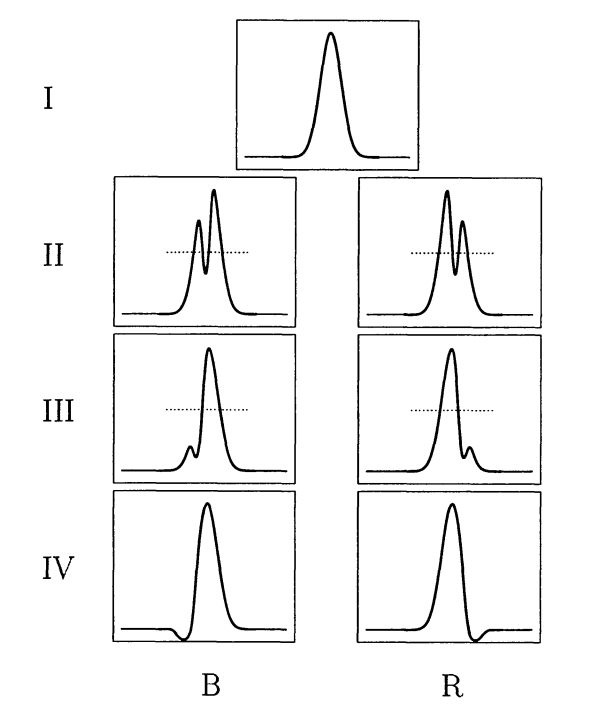
\includegraphics[scale=0.75]{figures/reipurth classes.png}
\caption{The morphology based classification scheme proposed by Reipurth et al. Depending on the location of the primary peak in relation to the secondary peak, the letters B and R were appended to the Roman numerals. They stand for blue-shifted and red-shifted respectively.}
\end{figure}

Published in 1996, Reipurth et al. studied the H$\alpha$ emission-line profiles of pre-main sequence stars using manual methods. In addition to identifying T Tauri stars and Ae\symbol{92}Be stars using high resolution spectra (R$\sim$50,000), the study focused on the morphological properties of P Cygni stars as well as the physical processes that generate them. The study notes the discovery of complex morphological profiles among the T Tauri, Ae\symbol{92}Be and P Cygni stars. 

The authors proposed a two dimensional classification scheme based on the relative height of a secondary peak compared to the primary peak, as well as whether the absorption line is blue or red shifted. The authors note the classification of 25\% symmetric profiles, 49\% blue shifted absorption profiles and 5\% P-Cygni profiles amongst the observed spectra. Of the spectra, 21\% fall into the red-shifted absorption category. In addition to this morphological classification, the authors also presented wind velocities of the samples with some stars recording extremely high velocities of $\sim$900km/s\cite{reipurth1996halpha}. 

The classification of P Cygni stars in this paper follow the scheme proposed by Beals in 1953\cite{1953PDAO....9....1B}. The authors have also presented a discussion comparing observed data to models in literature, particularly models that constrain mass, radii and photospheric temperatures. No specific model details for P Cygni stars were provided. Further catalogues of H$\alpha$ emission stars have been provided by Kohoutek and Wehmeyer (1997 and 1999). These catalogues contain 98 identified emission-line stars in the Northern Milky Way. These catalogues do not specifically identify P Cygni stars or inverse P Cygni stars\cite{kohoutek1999catalogue}.

The study of open clusters such as NGC 6611 and others have pushed our understanding of H$\alpha$ emission stars\cite{traven2015gaia}. Bonito et al. in particular\cite{bonito2013spectroscopic} note that for stars surrounded by active disks, the morphology of the emission lines could fall into categories such as symmetric with broad wings, asymmetric and in extreme cases, P Cygni and inverse P Cygni. The authors have used the classification scheme proposed by Reipurth et al. mentioned above and have adhered to the type I - IV scheme with B and R suffixes to denote blue-shifted and red-shifted emission lines respectively. 

Traven et al. presented a catalogue of H$\alpha$ emission stars in the Gaia-ESO survey. This survey is biased towards young open clusters and consequently, the authors note a relatively large proportion of H$\alpha$ emission spectra that were identified in this work. The authors note the identification of 3765 emission stars from a sample of 22,035 spectra from the Gaia-ESO survey. This work is notable as it uses a combination of empirical rules and automated techniques like spectral fitting to sort the H$\alpha$ emission spectra into eight distinct morphological categories: single–component emission, emission blend, sharp emission peaks, double emission, P-Cygni, inverted P-Cygni, self–absorption, and emission in absorption \cite{traven2015gaia}. The Gaia-ESO survey had conducted repeat observations of about half the identified H$\alpha$ emission stars. Thus the authors were able to comment on the temporal variability of these stars. The conclusion was that while some morphological categories exhibited stability of their spectral profiles over time, P-Cygni and self-absorption profiles may not. Supplementary information of these candidates from SIMBAD, VizieR and ADS were also provided. In addition to this data, the authors have provided wind velocity estimates based on the automated curve fitting procedure. The authors note that the identification, classification and characterisation of emission stars can be valuable for automatic pipelines in large surveys (e.g. GALAH), where they can pinpoint outliers when calculating general stellar properties and abundances. Additionally, they note that the identified stars can be used in studies of star formation processes, interacting binaries and related fields of stellar physics. 

This work draws several conclusions from this historical perspective,

\begin{enumerate}
\item These methods relied exclusively on visual inspection of spectra and manual methods to identify H$\alpha$ emission-line spectra. While this may have been a suitable approach in the past, it is extremely challenging to extend and scale these methods to data sets generated by million star all sky surveys in the modern era.

\item Morphology based classification approaches as demonstrated by Reipurth et al. and even Beals are important. It was demonstrated in Chapter 1 that the variety of spectral morphologies are hypothesised to be generated by distinct physical phenomena linked to the stellar disk and the gas that surrounds it.

\item Finally, these studies have identified P Cygni and inverse P Cygni (among other classes of spectra) as a subset of H$\alpha$ emission spectra. This work exploits this fact to its logical conclusion i.e. the probability identification of P Cygni and inverse P Cygni spectra can be increased if the search space and feature space of the raw data can be reduced from the complete DR3 catalog, to a much narrower subset of H$\alpha$ emission-line spectra during pre-processing. 
\end{enumerate}

\section{Recent Developments}

The increase in data availability via large scale spectroscopic surveys has necessitated and demanded the use of semi automated and fully automated detection and identification methods. More recently, these methods have included statistical analysis and machine learning. In general, machine learning approaches can fall into two categories; supervised and unsupervised learning. The former relies on the availability of a suitably robust set of training examples while the latter attempts to generalise and learn from unlabelled data\cite{hastie2009elements}. A full discussion and review of machine learning methods is beyond the scope of this thesis. Techniques and methods that are relevant to this research are presented in text in subsequent chapters. Chapter 4 in particular will present a more detailed discussion on methods that are relevant to this work. This section briefly reviews four recent approaches that rely on machine learning to detect and characterise H$\alpha$ emission-line spectra, their strengths and limitations.

\subsection{K-means Clustering on APOGEE Spectra}

K-means clustering is a well known unsupervised clustering algorithm.T he goal of this algorithm is to partition a set of observations into a predefined set of clusters. Each observation would belong to a cluster with the nearest mean which serves as the centroid or prototype of the cluster\cite{macqueen1967some}. Formally, given a set of $n$ observations such as \(x_1,x_2,...,x_n\) where each observation is a $d$ dimensional vector, the algorithm will partition the $n$ observations into $k$ sets $S=\{S_1,S_2,...,S_k\}$ such that within cluster variance is minimised. This objective can be represented as,

\begin{equation}
{\underset {\mathbf {S} }{\operatorname {arg\,min} }}\sum _{i=1}^{k}\sum _{\mathbf {x} \in S_{i}}\left\|\mathbf {x} -{\boldsymbol {\mu }}_{i}\right\|^{2}={\underset {\mathbf {S} }{\operatorname {arg\,min} }}\sum _{i=1}^{k}|S_{i}|\operatorname {Var} S_{i}
\end{equation}

where $\mu_i$ is the mean of the points in $S_i$. 

Using the identity,

\begin{equation}
    |S_{i}|\sum _{\mathbf {x} \in S_{i}}\left\|\mathbf {x} -{\boldsymbol {\mu }}_{i}\right\|^{2}=\sum _{\mathbf {x} \neq \mathbf {y} \in S_{i}}\left\|\mathbf {x} -\mathbf {y} \right\|^{2}
\end{equation}

It can be shown that this is equivalent to minimising the pairwise squared deviations of points belonging to the same cluster,

\begin{equation}
{\underset {\mathbf {S} }{\operatorname {arg\,min} }}\sum _{i=1}^{k}\,{\frac {1}{|S_{i}|}}\,\sum _{\mathbf {x} ,\mathbf {y} \in S_{i}}\left\|\mathbf {x} -\mathbf {y} \right\|^{2}
\end{equation}

APOGEE, which is part of the Sloan Digital Sky Survey (SDSS) is a high resolution spectroscopic survey (R$\sim$22,500)\cite{eisenstein2001spectroscopic}\cite{blanton2017sloan}. In the absence of labelled training samples in the APOGEE survey Garcia-Dias et al. used k-means to cluster similar spectra into distinct groups\cite{garcia2018machine}. Each spectrum produced by APOGEE was treated as a $d$-dimensional vector. The number of observations $n$ was the number of spectra generated by APOGEE which was approximately 150,000. $k$ was set to 50. The authors note that they were able to separate dwarfs, sub-giants, RC and RGB stars. The authors note that the approach is sensitive to initialisation and thus sensitive to the number of clusters $k$. One major limitation of this approach is that a discrete classification in the flux space does not result in a neat organisation in the parameters' space. The other limitation being the use of manual sorting of clusters that reduced the number of clusters from 50 to 9. This implies that certain spectra were incorrectly clustered by the k-means algorithm. The authors were unable to cluster H$\alpha$ emission spectra using this method. 

The primary conclusion that can be drawn from this work is that k-means clustering, while robust on more traditional machine learning tasks may perform poorly if it is used to cluster and ultimately classify morphologically similar spectra such as P Cygni and inverse P Cygni. A methodology that relates the flux space, and consequently the morphology of the spectrum, to a parameter space may perform better than k-means. 

\subsection{Automated and Manual Methods on LAMOST Spectra}

The LAMOST survey is a low resolution spectroscopic survey with 10 million Milky Way stars as potential survey candidates. Zhang et al. were able to use a training and test set (labelled spectra) comprising 5,915 samples for spectral classification. This training set was based on data released by Hou et al.\cite{hou2016catalog} who developed the data set by using a combination of empirical rules and visual examination of 10,000 LAMOST spectra. The existence of labelled data including seven P Cygni and inverse P Cygni spectra identified by Hou et al. was exploited for supervised machine learning algorithms. 

As such, 10 different supervised learning methods were then applied to this data set including including KNN (K-Nearest Neighbor), RF (Random Forest), AdaBoost, Naive Bayes (MultinomialNB, GaussianNB, BernoulliNB), logistic regression, SVM (Support Vector Machine) and Artificial Neural Network (Single-hidden Layer, Three-hidden Layer)\cite{zhang2021catalog}. A comparison of the performance of these methods were not provided by the author. A detailed discussion of these methods is omitted as it would be beyond the scope of this thesis. 

However they note that the k-nearest neighbour and random forest methods outperformed all other methods. These two supervised machine learning models were then applied to 498,588 spectra resulting in 56,574 potential H$\alpha$ emission candidates. These candidates were then visually inspected with a final candidate list of 30,048 H$\alpha$ emission spectra. A significant drawback of this approach is the reliance on manual visual inspection of spectra in building the training set as well as during classification of the identified potential H$\alpha$ emission spectra. A labelled training set with clearly identified P Cygni and inverse P Cygni spectra does not currently exist for GALAH DR3 and thus none of these methods can be extended to DR3. In Chapter 4, this work will demonstrate an automated method that generates a data set which does not rely on manual visual inspection.

\subsection{t-SNE and DBSCAN on GALAH DR1}

As discussed previously, a stellar spectrum of vector length $d$ (a wavelength grid of size $d$), can be used to create a vector space of minimum dimensionality equal to $d$. In the case of GALAH DR1 this value is $\sim$4500. Conducting computational operations such as clustering and classification on a higher dimensional vector space of size $\sim$4500 can be challening as it introduces significant computational overheads. In addition to the previously mentioned curse of dimensionality, researchers would also face practical limitations due to the computational intractability of working on higher dimensional vector spaces. It is often helpful to transform the data from a high-dimensional space to a low-dimensional space ensuring that meaningful features of the original data are preserved. In the case of P Cygni and inverse P Cygni spectra, these meaningful properties would presumably include some information about the morphology of the spectrum although this may not be guaranteed. This work will revisit this in detail in Chapter 5.

Given a total feature space (and consequently a total search space) that is made up of $n$ spectra samples of length $d$, dimensionality reduction offers an attractive approach to grapple with the curse of dimensionality and high computational complexity. Principal component analysis (PCA) is arguably the most well known dimensionality reduction technique. However, PCA may not be suitable in the context of GALAH DR1 and certainly DR3 since these data sets are biased towards non-emission line spectra. Thus a PCA led approach may select features that represent the absorption-line, while emission-line features may not be considered a principal component. This hints at a possible outlier or anomaly detection based approach to emission-line spectra identification. This work will revisit this idea in Chapter 6.

More recent and novel dimensionality reduction techniques such as t-distributed stochastic neighbour embedding (t-SNE)\cite{van2008visualizing} have been used on spectral data from GALAH DR1\cite{traven2017galah}. Given a vector of size $d$, the application of the t-SNE algorithm will project this vector space onto a 2-dimensional vector space. The distances between data points on this 2-dimensional vector space can then be used to cluster similar data points into similar groups using a variety of popular clustering methods such as DBSCAN\cite{ester1996density} or HDBSCAN\cite{campello2013density}. A detailed discussion of this technique and its tuitability to this work is presented in Chapter 5.

\begin{figure}[!htb]
\centering
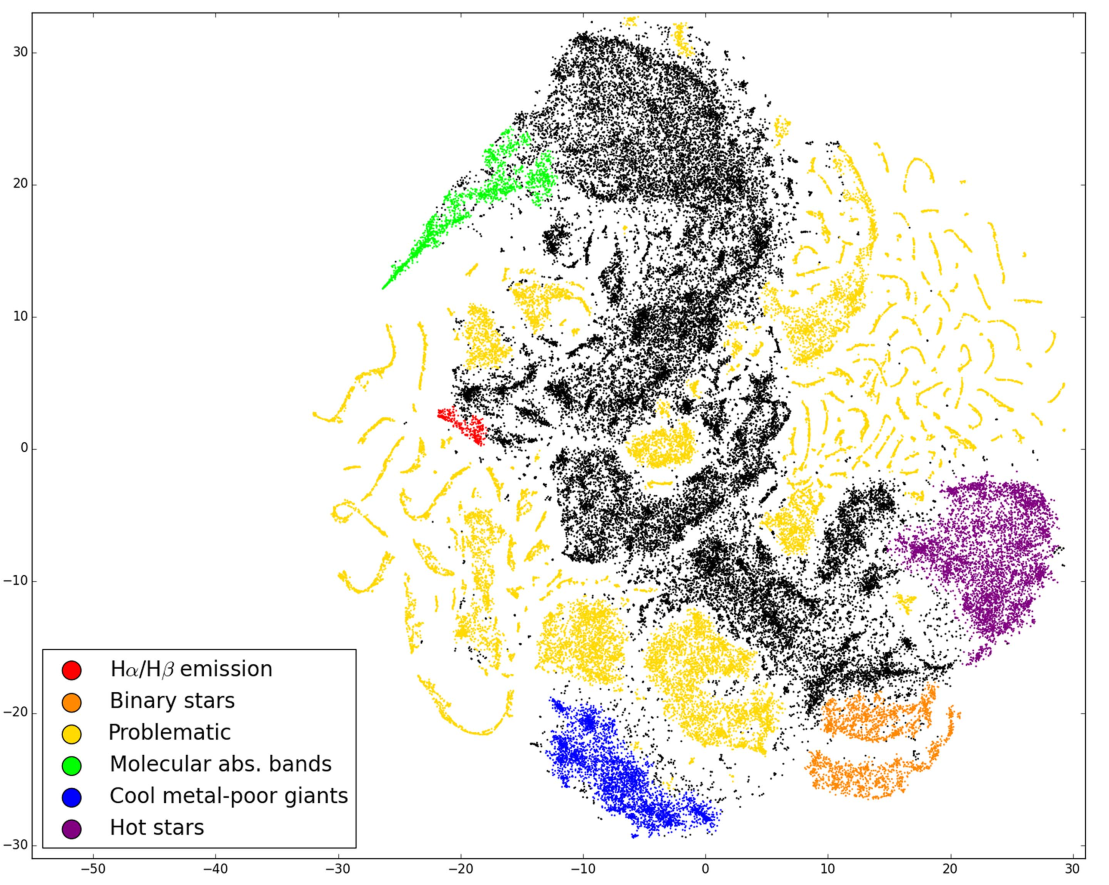
\includegraphics[scale=0.40]{figures/tsne traven.png}
\caption{The t-SNE plot with classified regions reproduced from Traven et al.\cite{traven2017galah}. The x and y axes do not have a physical meaning but serve as spanning vectors for the 2-dimensional projection space.}
\end{figure}

Using this method, Traven et al. classified six distinct stellar types and identified H$\alpha$ and H$\beta$ emission-line spectra in GALAH DR1. These spectra were further examined and 18 P Cygni spectra were identified. The identification of P Cygni spectra was a sub-component of a broader study of stellar types in GALAH DR1. The authors note that the number identified was lower than expected. The method was not able to clearly separate P Cygni spectra from double peaked spectra, emission superimposed on absorption and other emission candidates. When examining the t-SNE plot above, it is clear that the authors were not able to distinctly separate the H$\alpha$ emission stars as a distinct cluster from the unclassified region (black). This thesis will revisit this study in subsequent chapters and demonstrate a data driven method of separating P Cygni spectra from the aforementioned categories that can overcome some of the limitations mentioned above.

\subsection{Autoencoders on GALAH DR3}

An autoencoder (AE) is a type of artificial neural network (ANN) that takes input data and reduces it to a pre-selected number of "latent features" that inhabit a low-dimensional vector space known as the latent space. The latent space can capture important features that exist in the original $d$-dimensional vector space. By processing $n$ samples of $d$-dimensional vectors, the autoencoder can then learn the latent space representation of the higher dimensional features. This is known as encoding. In the next portion of the network, the network then attempts to recover the original data from the latent vector space. The process that reduces a $d$-dimensional vector and vector space to a vector space of size $p$<$d$ is a dimensionality reduction process similar to PCA or t-SNE. The portion of the network that takes a $p$-dimensional vector from the latent space and projects it back to a $d$-dimensional vector space is essentially the inverse process of the dimensionality reduction procedure. This is known as a decoder. Since the original data is generated from the latent space, autoencoders fall into a class of ANNs called generative models (generative ANNs). Note that the latent space for an autoencoder is discrete. ANNs that can generate continuous latent spaces in this manner are known as variational autoencoders (VAEs) and are beyond the scope of this work. 

Autoencoders are widely used in anomaly detection applications\cite{sakurada2014anomaly}. If the autoencoder model is trained on non-anomalous data ("normal" data), the model will learn the latent space representation of non-anomalous data. subsequently, if an anomalous data point is passed through the model, the autoencoder will attempt to generate this data from the latent space representation it has learned. Since the learned model was trained on non-anomalous data, the autoencoder will generate an inaccurate representation of the anomalous data. This leads to a significant prediction error between the generated anomalous data and the true anomalous data. This process can be exploited to detect time-series as well as non time-series anomalies in data.

The GALAH survey is a general all-sky survey that can be expected to generate a significantly higher proportion non-anomalous spectra. Since DR3 is not biased towards young, violent, hot stars or stellar nurseries, we expect a significantly higher proportion of spectra to show "normal" (non-anomalous) H$\alpha$ line profiles and indicate absorption. In this regime, an H$\alpha$ emission, and consequently, P Cygni and inverse P Cygni spectra are rare and anomalous. If an autoencoder is trained on "normal looking" spectra which do not show emission lines near H$\alpha$, it can be sensitive to H$\alpha$ emission-line spectra. 

\begin{figure}[!htb]
\centering
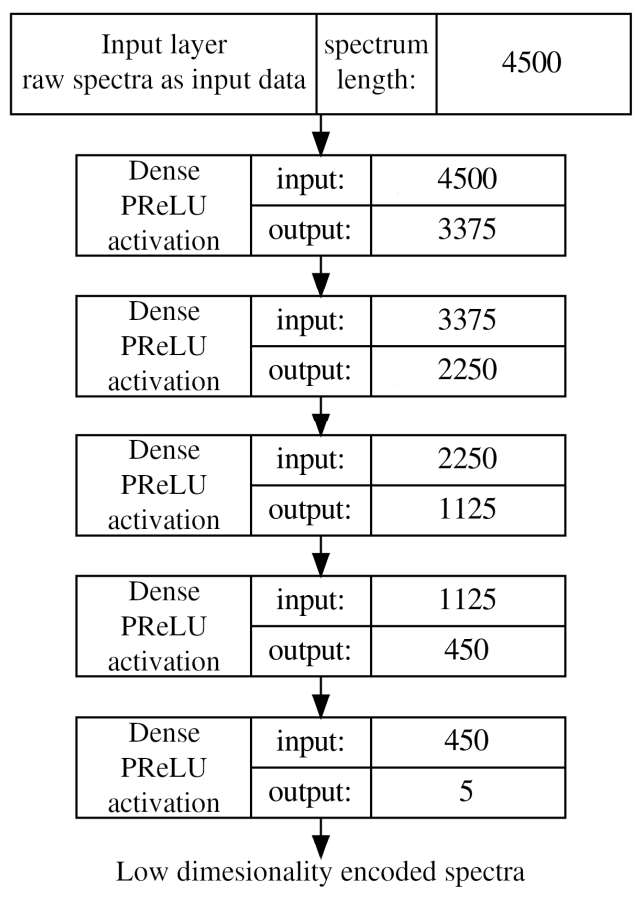
\includegraphics[scale=0.45]{figures/autoencoder.png}
\caption{An autoencoder architecture capable of detecting H$\alpha$ candidates from DR3. Reproduced from Čotar et al.\cite{vcotar2021galah}}
\end{figure}

This methodology was exploited by Čotar et al. to detect H$\alpha$ emission-line spectra in DR3 and other surveys\cite{vcotar2021galah}. Hyper-parameter tuning is both an art and a science and requires a trial and error approach. The authors chose a network architecture that reduces a $d$-dimensional DR3 spectrum to a $p$-dimensional latent space representation. Here, $d$ = 4500 while $p$ = 5. The intervening layers and the final architecture that is capable of detecting "anomalous" H$\alpha$ emission spectra is presented below. An introduction to the H$\alpha$ emission-line spectra that were detected using this method was presented in Chapter 2. The authors did not further classify and detect P Cygni and inverse P Cygni candidates using this method. This thesis makes extensive use of this data to identify and characterise P Cygni and inverse P Cygni spectra using data driven methods. This methodology is discussed in detail in the next chapter. 

